\section{Results}

\subsection{Proof of convergence history}
Pleas see Appendix
\subsection{Table of final lift and drag coefficients and related forces}
\begin{table}[H]
	\centering
	\begin{tabular}{|c|c|c|} \hline
		\centering
		\textbf{Case}       & $C_L$ [-]   & $C_D$ [-]    \\ \hline
		10         & 0.143 & 0.075 \\ \hline
		20         & 0.341 & 0.174 \\ \hline
		30         & 0.545 & 0.371 \\ \hline
		Adapted 20 & 0.342 & 0.173 \\ \hline
	\end{tabular}
\end{table}

\subsection{Plot of lift and drag and L/D vs. AOA with peak L/D identified}

\begin{figure}[H]
 \centering
 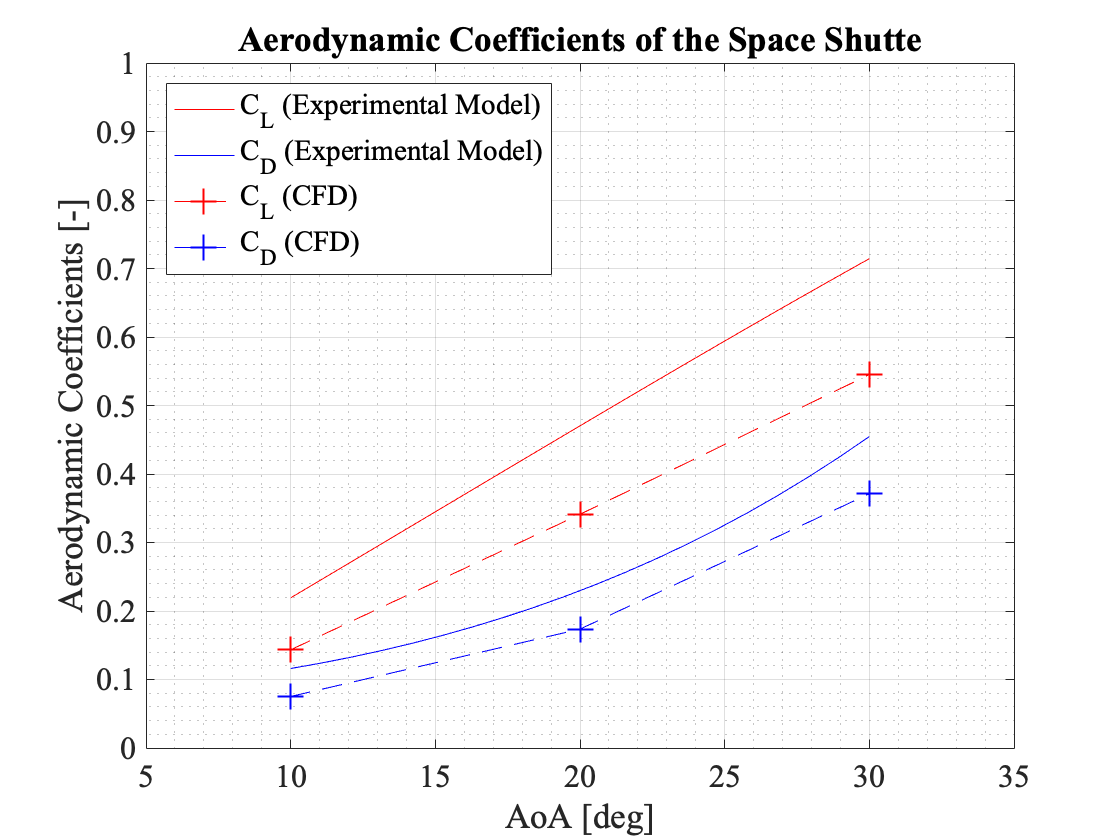
\includegraphics[width=0.7\textwidth]{matlab_images/aero_coeff_comp.png}
 \caption{Comparison of the $C_L$ and $C_D$ results from the experimental model and the CFD cases ran}
 \label{fig: aero_coeff_comp}
\end{figure}

\begin{figure}[H]
 \centering
 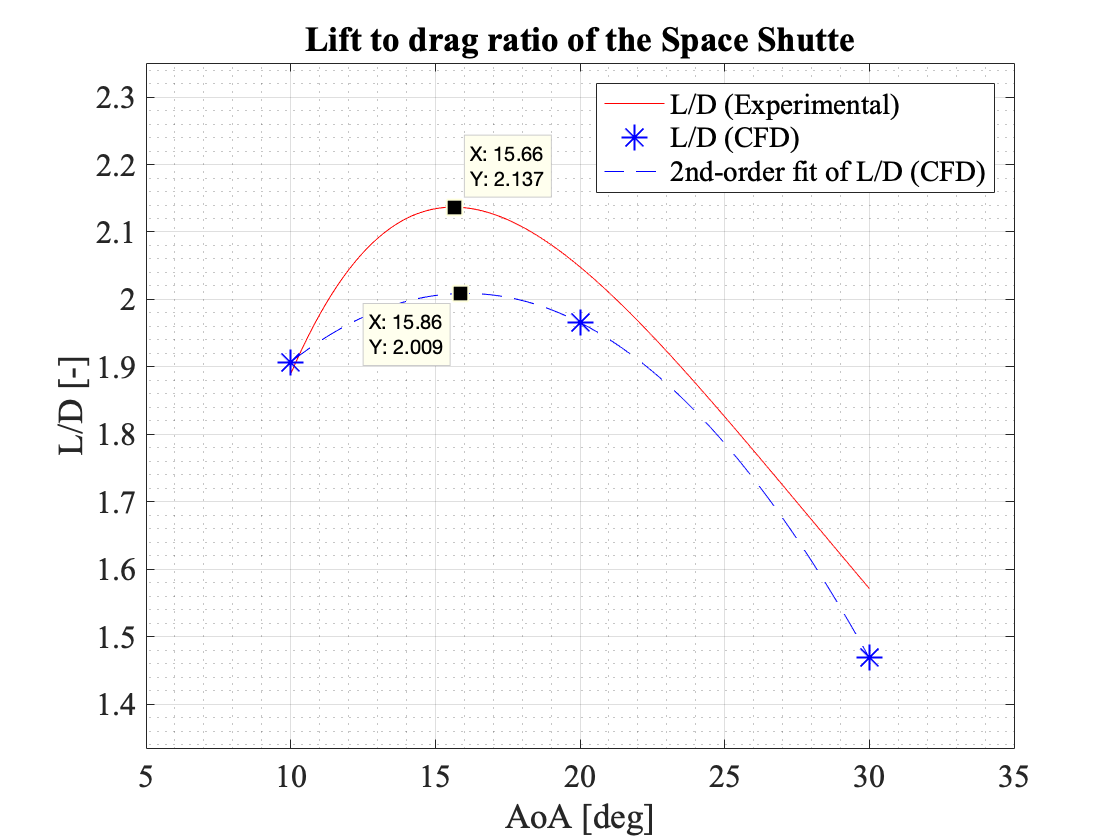
\includegraphics[width=0.7\textwidth]{matlab_images/L2D.png}
 \caption{Comparison of the lift-to-drag ratios from the experimental model and the CFD cases ran}
 \label{fig: l2d}
\end{figure}

\subsection{Pressure and temperature contours with streamlines}

\subsubsection{AoA = 10$^\circ$}
\begin{figure}[H]
 \centering
 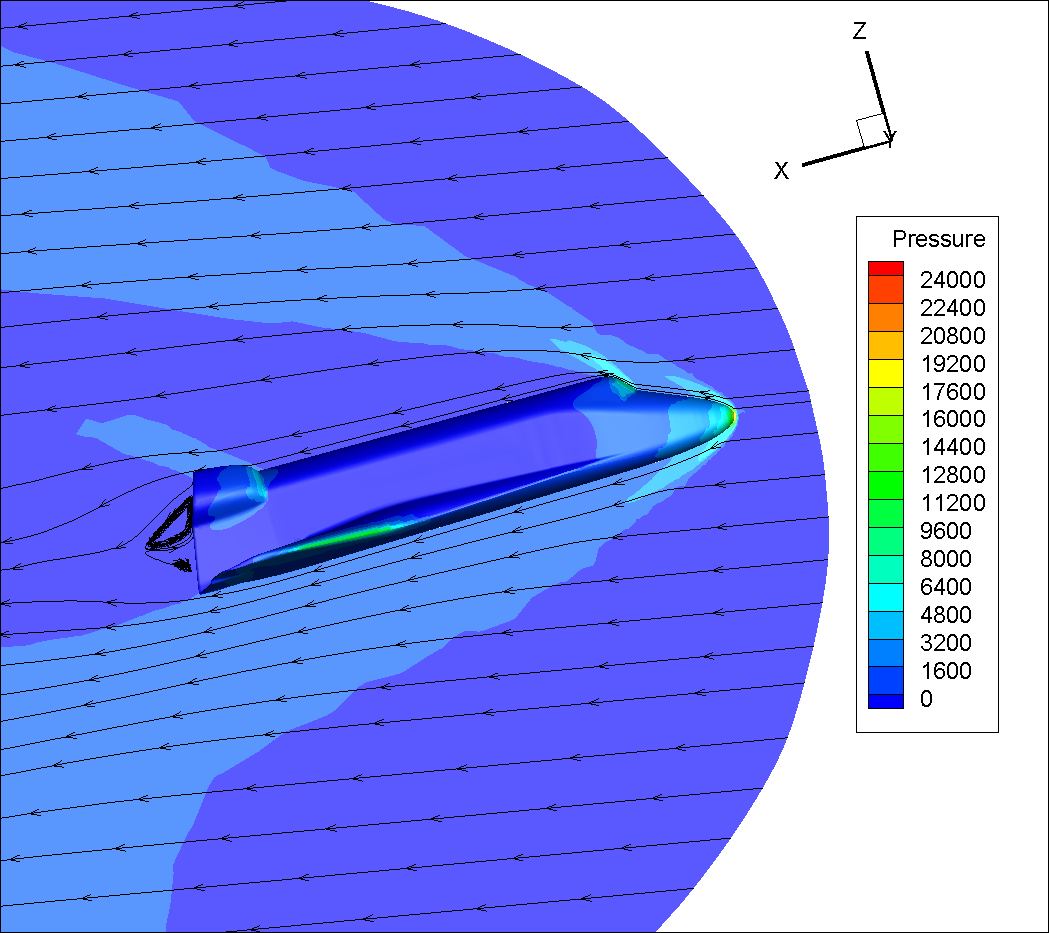
\includegraphics[width=\textwidth]{report_images/10_sym_pressure_contour.png}
 \caption{Pressure contour at the symmetry plane of the orbiter at 10 degs AoA}
 \label{fig: 10_sym_pressure_contour}
\end{figure}

\begin{figure}[H]
 \centering
 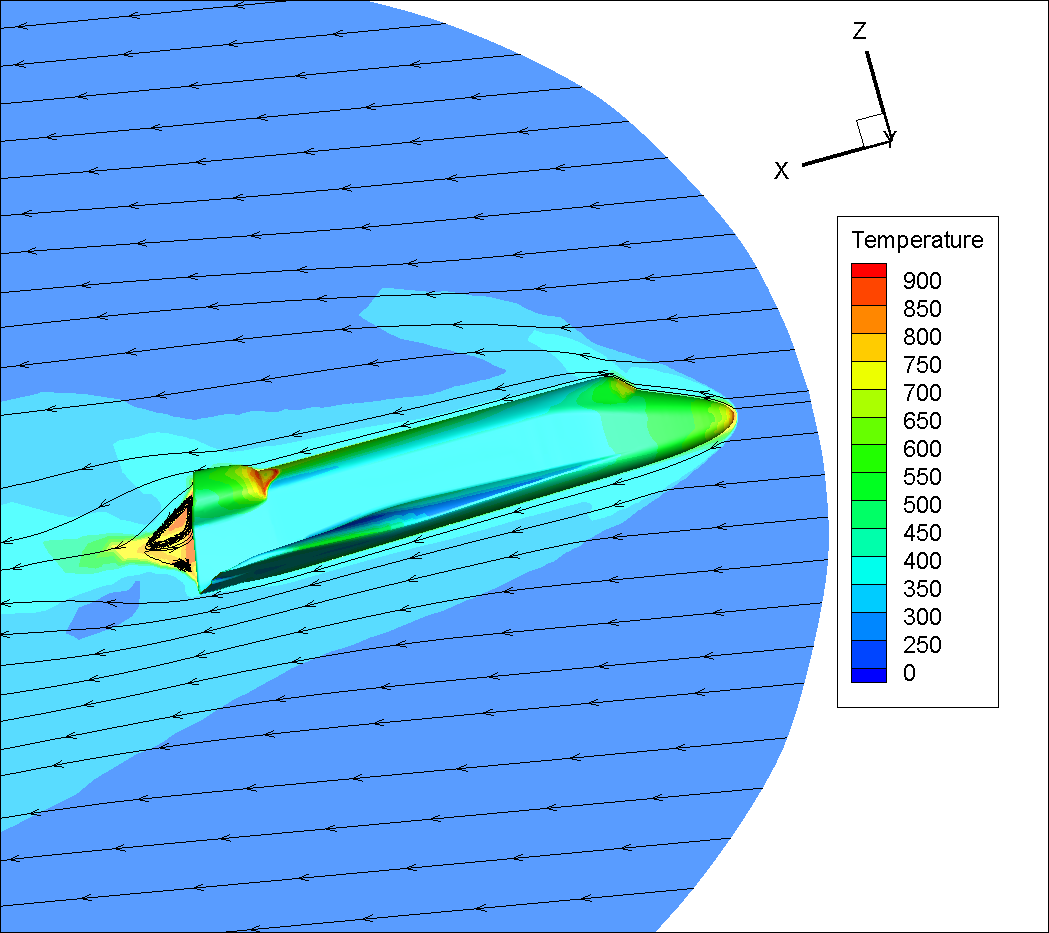
\includegraphics[width=\textwidth]{report_images/10_sym_temp_contour.png}
 \caption{Temperature contour at the symmetry plane of the orbiter at 10 degs AoA}
 \label{fig: 10_sym_temp_contour}
\end{figure}

\subsubsection{AoA = 20$^\circ$}
\begin{figure}[H]
 \centering
 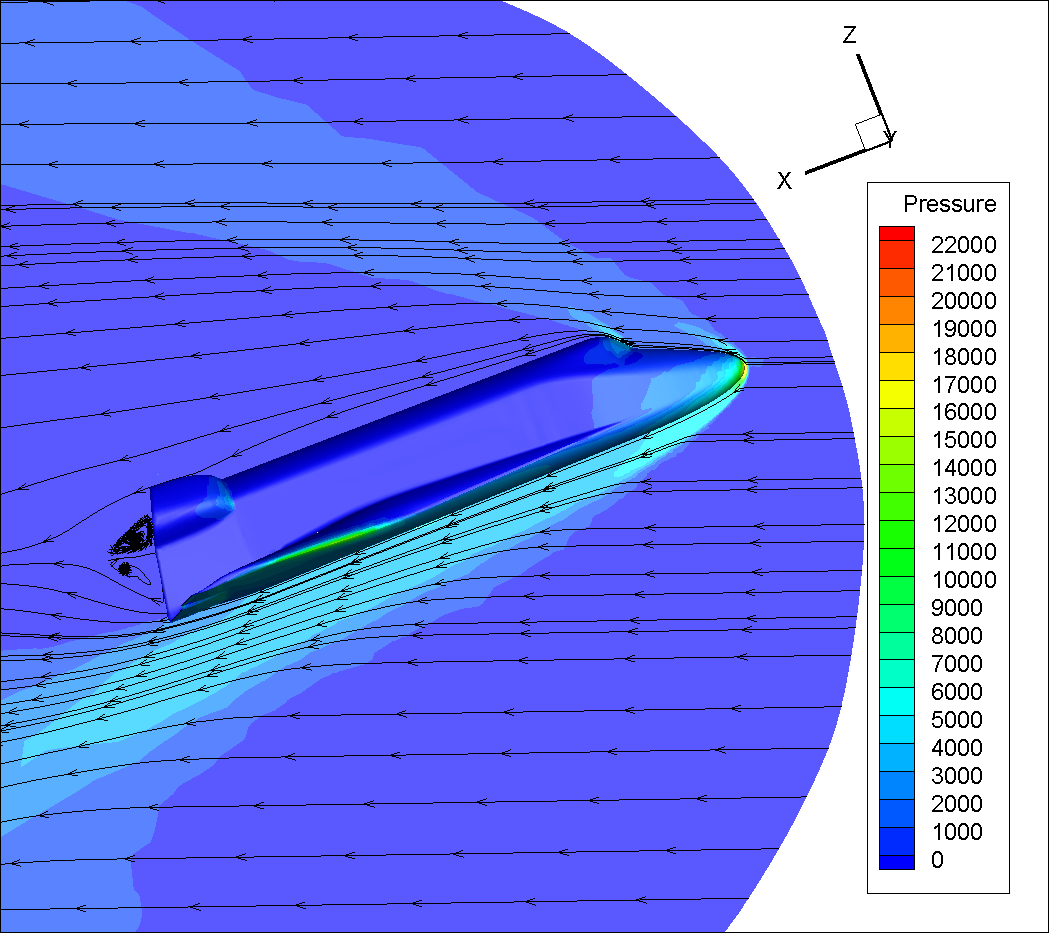
\includegraphics[width=\textwidth]{report_images/20_sym_pressure_contour.png}
 \caption{Pressure contour at the symmetry plane of the orbiter at 20 degs AoA}
 \label{fig: 20_sym_pressure_contour}
\end{figure}

\begin{figure}[H]
 \centering
 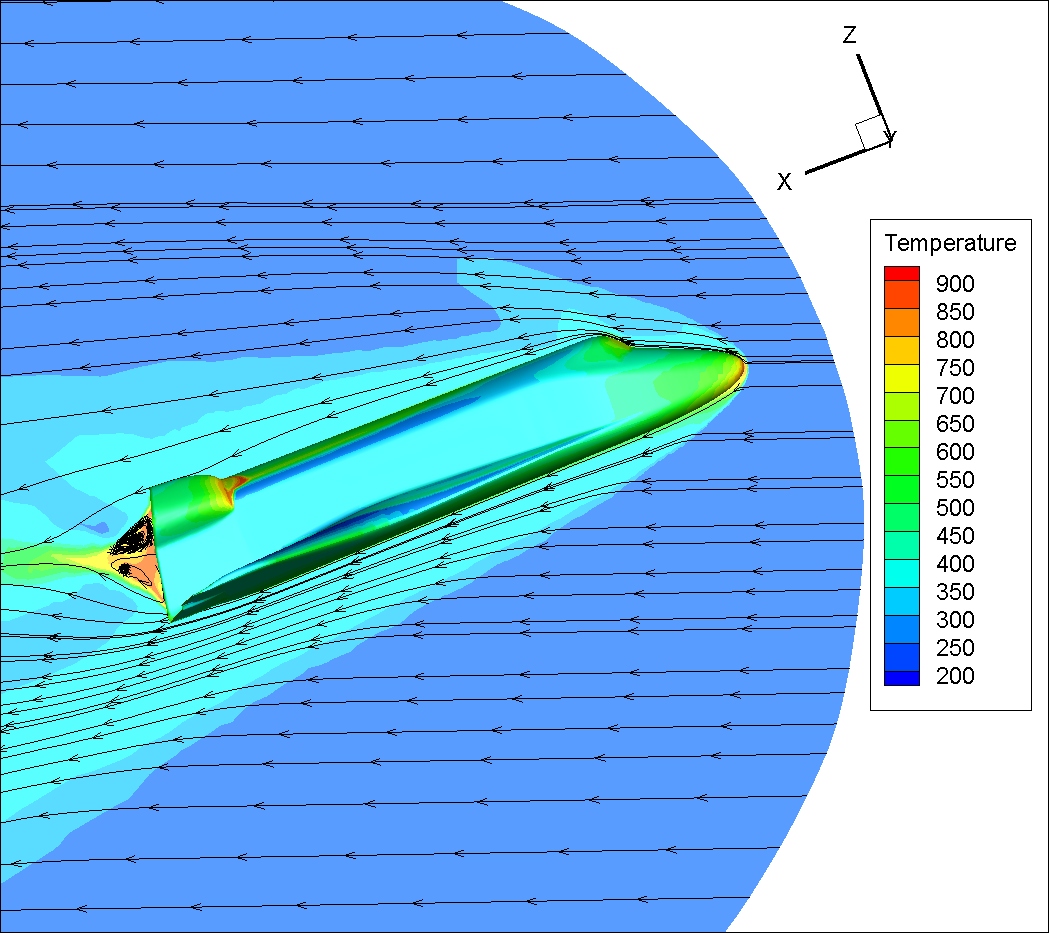
\includegraphics[width=\textwidth]{report_images/20_sym_temp_contour.png}
 \caption{Temperature contour at the symmetry plane of the orbiter at 20 degs AoA}
 \label{fig: 20_sym_temp_contour}
\end{figure}

\subsection{Results of grid adaptation}

\subsubsection{Side by side of contour plots}

\subsubsection{Side by side of mesh}

\subsubsection{Table of force coefficients}

\subsubsection{Fluent settings used to adapt grid}